\documentclass{beamer}
\usepackage{othelloboard}
\usepackage{tikz} % othelloboard not compatible with beamer (i think) so we use TikZ to show images

\usetheme{Boadilla}


\title{Première Presentation}
\subtitle{OTHELLO}
\author{Groupe 11}
\date{16 01 2025}

\begin{document}



\begin{frame}
  \titlepage
\end{frame}


\begin{frame}
  \frametitle{Sommaire}
  \tableofcontents
\end{frame}

\section{Contexte}
%\subsection{sub a}
\section{Explication du sujet}
\subsection{Règles}
\subsection{Structures de données}
\subsection{Algorithmes utilisés}
\section{Besoins visés}
\section{Agenda prévisionnel}



\begin{frame}
  \frametitle{Contexte}
  Pour ce projet, nous allons travailler en Python sur le jeu de plateau Othello.\\
  Othello (ou Reversi) (Othello est une marque déposée) se joue à deux joueurs, sur un plateau carré de 8x8 cases.\\
  Chaque joueur possède des pions de couleur blanche ou noire.\\
  Notre but ici sera d'implémenter ce jeu en langage python, et de donner une interface graphique et des commandes additionnelles à l'utilisateur.\\
\end{frame}


\begin{frame}
  \frametitle{Explication du sujet - Règles}
  Othello se joue sur un plateau unicolore de 64 cases: l'othellier.\\
  Les deux adversaires jouent avec 64 pions de couleur blanche d'un côté et noire de l'autre.\\
  Au tout début de la partie, quatre pions sont placés au centre du plateau: deux pions noirs en E4 et D5, et deux pions blancs en E5 et D4.\\
  (cf. diapositive suivante pour une représentation du jeu dans son état initial)\\
  Les cases de l'othellier sont numérotées par les lettres A à H pour les colonnes, et par les chiffres 1 à 8 pour les lignes.
\end{frame}

\begin{frame}
  \frametitle{Explication du sujet - Règles}
  % commented because there is a problem using beamer with othello package :(
  % \begin{center}
  %     \begin{othelloboard}{8} % 8x8 board
  %         \othello{4}{4}{black} % Place a black piece at (4,4)
  %         \othello{4}{5}{white} % Place a white piece at (4,5)
  %         \othello{5}{4}{white} % Place a white piece at (5,4)
  %         \othello{5}{5}{black} % Place a black piece at (5,5)
  %     \end{othelloboard}
  % \end{center}
  \begin{center}
    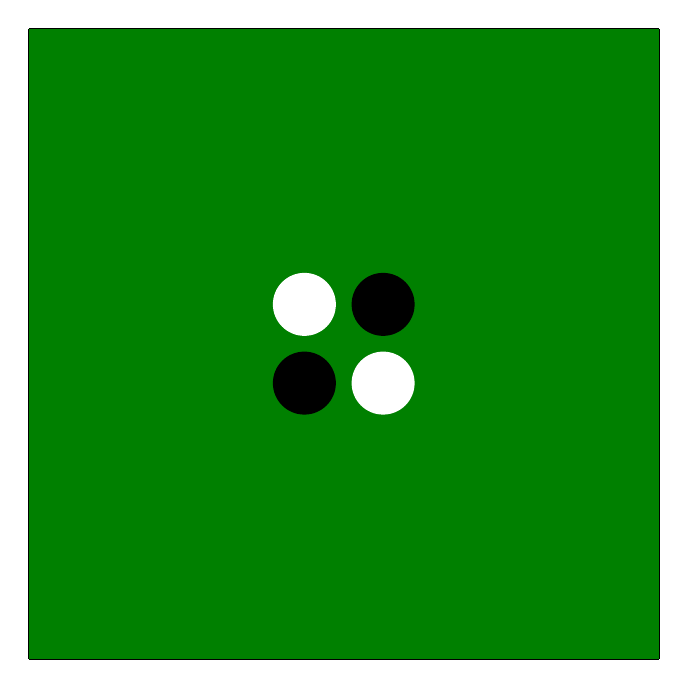
\begin{tikzpicture}
      % Draw the board
      \draw[thick] (0,0) grid (8,8);
      \foreach \x in {0,1,...,7} {
        \foreach \y in {0,1,...,7} {
          \fill[green!50!black] (\x,\y) rectangle (\x+1,\y+1);
        }
      }

      % Place the pieces
      \fill[black] (3.5,3.5) circle (0.4);
      \fill[white] (3.5,4.5) circle (0.4);
      \fill[white] (4.5,3.5) circle (0.4);
      \fill[black] (4.5,4.5) circle (0.4);
    \end{tikzpicture}
  \end{center}
\end{frame}


\begin{frame}
  \frametitle{Explication du sujet - Règles}
  Les joueurs jouent chacun leur tour, en commençant par le joueur aux pions noirs.\\
  Ils doivent capturer les pions de leur adversaire à chaque tour.\\
  Si le joueur ne peut pas capturer de pion, il passe son tour.\\
  Un pion placé doit être adjacent à au moins un autre pion (de même couleur ou de couleur adverse) dans sa ligne, colonne ou diagonale.
\end{frame}


\begin{frame}
  \frametitle{Explication du sujet - Règles}
  Une capture se produit lorsque le joueur dont c'est le tour place un pion qui enferme un alignement (en colonne, ligne, ou diagonale) de pions adverses (l'autre extrémité étant fermée au cours d'un tour précédent).\\
  En plaçant son pion, le joueur retourne les pions qu'il capture, les changeant en sa couleur.\\
  Si le pion posé permet de capturer plusieurs alignements à la fois, le joueur capture tous ces pions adverses.\\
  Par contre, en les retournant, ces pions ne permettent pas de capture, même si ils encadrent des pions adverses.
\end{frame}


\begin{frame}
  \frametitle{Explication du sujet - Règles}
  Le jeu se termine lorsqu'aucun des deux joueurs ne peut poser de pion, ou que l'othellier n'a plus aucune case vide.\\
  On compte le nombre de pions de chaque couleur sur le plateau pour déterminer le vainqueur: le joueur ayant le plus de pions de sa couleur présents sur l'othellier.
\end{frame}


\begin{frame}
  \frametitle{Explication du sujet - Structures de données}
  lorem ipsum
\end{frame}


\begin{frame}
  \frametitle{Explication du sujet - Structures de données}
  Bitboards\\
  + mask (pour le board entier)\\
  + bitsB (pour les pions noirs)\\
  + bitsW (pour les pions blancs)\\
  + bitsM (pour les pions modifiés au cours du dernier tour)
\end{frame}


\begin{frame}
  \frametitle{Explication du sujet - Structures de données}
  Operations\\
  + ...\\
  + (si on en utilise mais pas sûr)\\
\end{frame}


\begin{frame}
  \frametitle{Explication du sujet - Algorithmes utilisés}
  + Line Move Filters : liste de Legal Moves (dans une direction)\\
  + Surround Capture / Flip Enemy Neighbours of Last Move % idk lequel ou un mix des deux, en gros, flip les pions capturés quand ils sont encadrés
\end{frame}



\begin{frame}
  \frametitle{Besoins visés}
  Premièrement, nous allons lister ici les besoins nécessaires au bon fonctionnement du jeu:\\[0.5cm]
  \begin{columns}[t] % "t" aligns content at the top; use "c" for center or "b" for bottom
    \column{0.5\textwidth} % Adjust width (e.g., 0.5 for half the slide)
    % Left side content
    \textbf{Jeu} \\
    \begin{itemize}
      \item Plateau de jeu (Othellier) (F.27, F.41, F.42, F.43)
      \item Initialiser une partie (F.???)
      \item Jouer un coup (F.28)
      \item Abandon (F.30)
      \item Fin de partie (F.36)
    \end{itemize}
    \column{0.5\textwidth} % Adjust width
    % Right side content
    \textbf{A actualiser en permanence} \\
    \begin{itemize}
      \item Documentation (F.5)
      \item Tests (F.6)
      \item Bugs fixés (F.7)
    \end{itemize}
  \end{columns}
\end{frame}



\begin{frame}
  \frametitle{Besoins visés}
  Ensuite, voici des besoins plus spécifiques, à implémenter dans un second temps:\\[0.5cm]
  \begin{columns}[t]
    \column{0.5\textwidth}
    % Left side content
    \textbf{Options en lignes de commande} \\
    \begin{itemize}
      \item Nom de l'exécutable (F.14)
      \item Usage (F.15)
      \item Help (F.16)
      \item Version (F.17)
      \item Taille du plateau (F.20)
    \end{itemize}
    \column{0.5\textwidth}
    % Right side content
    \textbf{Interface utilisateur} \\
    \begin{itemize}
      \item Interface en ligne de commande (F.25)
      \item Historique (F.29, F.39, F.33, F.34)
      \item Reset (F.35)
      \item Sauvegarder partie (F.32, F.38)
      \item Rejouer une partie (F.37)
      \item Configuration (F.40)
    \end{itemize}
  \end{columns}
\end{frame}


\begin{frame}
  \frametitle{Besoins visés}
  Dans un troisième temps, nous précisons les besoins précédents et ajoutons les bases pour un joueur IA:\\[0.5cm]
  \begin{columns}[t]
    \column{0.5\textwidth}
    % Left side content
    \textbf{Précisions} \\
    \begin{itemize}
      \item Performances (F.8)
      \item Internationalisation (F.13)
      \item Verbose (F.18)
      \item Debug (F.19)
      \item Mode blitz (F.21, F. 22)
      \item Mode Contest (F.23)
      \item Affichage des messages (F.31)
    \end{itemize}
    \column{0.5\textwidth}
    % Right side content
    \textbf{Joueur IA} \\
    \begin{itemize}
      \item Mode IA (F.24)
      \item Heuristique(s) (F.51)
      \item Minimax (F.52)
      \item Profondeur de recherche (F.56)
      \item Calcul des libertés (F.58)
      \item Calcul des pierres stables (F.59)
    \end{itemize}
  \end{columns}
\end{frame}


\begin{frame}
  \frametitle{Besoins visés}
  Finalement, nous ajoutons l'interface graphique et améliorons notre IA:\\[0.5cm]
  \begin{columns}[t]
    \column{0.5\textwidth}
    % Left side content
    \textbf{Joueur IA} \\
    \begin{itemize}
      \item Heuristiques (F.51)
      \item AlphaBeta pruning (F.53)
      \item Exploration préliminaire (F.54)
      \item MCTS (F.55)
      \item Choix des heuristiques (F.57)
      \item Temps de réflexion (F.60)
    \end{itemize}
    \column{0.5\textwidth}
    % Right side content
    \textbf{Interface graphique} \\
    \begin{itemize}
      \item Interface graphique (F.26, F.48)
      \item Fonctions de base (F.44)
      \item Menu FILE (F.45)
      \item Menu GAME (F.46)
      \item Menu ABOUT (F.47)
      \item Affichage des coups joués (historique) (F.49)
      \item Configuration nvelle partie (F.50)
    \end{itemize}
  \end{columns}
\end{frame}



\begin{frame}
\frametitle{Agenda prévisionnel}
Lorem ipsum dolor sit amet, consectetur adipisicing elit, sed do eiusmod tempor incididunt ut labore et dolore magna aliqua.
\end{frame}


\end{document}